%!TEX program = xelatex
% 完整编译方法 1 pdflatex -> bibtex -> pdflatex -> pdflatex
% 完整编译方法 2: xelatex -> bibtex -> xelatex -> xelatex
\documentclass[lang=cn,11pt]{elegantpaper}
\usepackage{url}
\usepackage{booktabs}
\usepackage{multirow}
\usepackage{geometry}
\usepackage{longtable}
\usepackage{pdfpages}
\title{基于卷积神经网络和迁移学习的图像识别模型}

% 不需要版本信息, 直接注释即可
% \version{0.07}
% 不需要时间信息的话, 需要把 \today 删除. 
\date{}


% 如果想修改参考文献样式, 请把这行注释掉
% \usepackage[authoryear]{gbt7714}  % 国标

\begin{document}


\newpage
\maketitle

\vspace{-25pt}
\begin{abstract}



\end{abstract}
\keywords{}
	
\tableofcontents
\thispagestyle{empty}
\newpage
\normalsize
\pagenumbering{arabic}


\section{模型实践与改进}

我们使用了sklearn中ensemble类里的AdaBoostClassifier类. 数据集选用了UCI数据集中的IRIS数据集. IRIS数据集是一个花卉分类数据集, 其中给出了标记好的三种花卉(Iris Setosa-山鸢尾, Iris Versicolour-杂色鸢尾, 以及Iris Virginica-维吉尼亚鸢尾), 以及其所对应的四个特征(花萼长度, 花萼宽度, 花瓣长度, 花瓣宽度). 我们的任务是学习一个函数, 使得其通过输入这三种花其中的某一种的一个植株的这四个参数, 能够判断出这个植株是哪一种花. 这是一个典型的分类问题, IRIS数据集也是应用广泛的数据分类数据集. 我们首先将数据集分为训练集与测试集两部分进行训练.

\begin{figure}[hbt]
\centering
  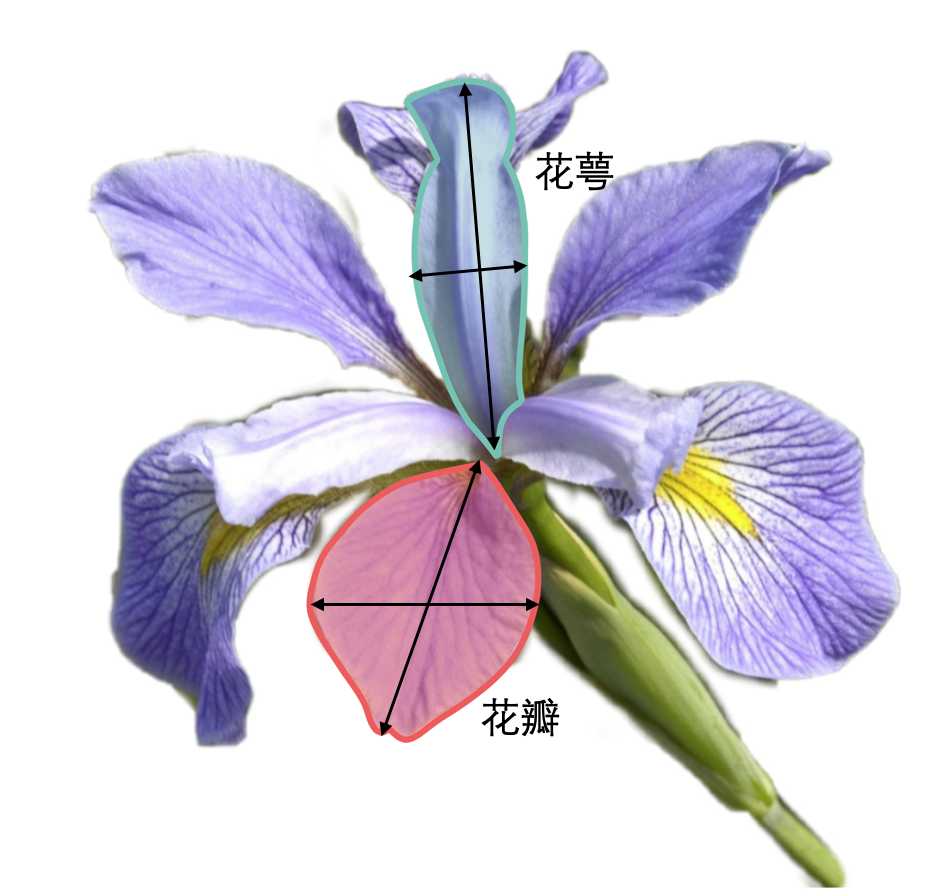
\includegraphics[width=0.75\textwidth]{flower.png}
  \caption{弗吉尼亚莺尾的花萼与花瓣示意图\label{fig:VGflower}}
\end{figure}


\subsection{决策树弱学习机}

我们的模型采用了50个决策树作为弱学习机, 采用了默认的学习率Sklearn的AdaboostClassifier能够全自动地帮我们完成优化损失函数. 我们在测试集上获得了87.6\%的准确率. 这并不是一个多么令人可喜的结果. 我们希望了解我们的模型哪里出了问题. 于是我们尝试了可视化模型.

我们尝试可视化了我们模型的分类边界. 不过由于四维的数据可视化起来比较困难. 我们又只在其中的两个特征(两个长度)上使用相同的方法与参数训练出来了一个学习机, 我们觉得这样的简化版学习机可以很好地解释学习机的限制以及学习的过程中发生了什么. 而通过可视化我们的确发现了我们模型中致命的问题.

从图上也可以看出这两个特征可以很好的将A类山莺尾与B类杂色莺尾、C类弗吉尼亚莺尾分开, 但是对于B、C类之间的分类做的很差. 除了这两个特征我们需要更多的信息去区分B、C类. 我们推测这个原因并不是我们的学习机的问题, 通过另外的两维特征我们应该可以在一定程度上解决这个问题. 因为其更像是某个高维空间的散点在这个低维空间上的投影.

另外一个问题是我们发现我们的弱学习机的集成依旧保持着弱学习机本来的分类边界的特点, 是一个超级纵横学习机, 本质上没有突破纵横学习机的限制. 分类的边界属于横平竖直. 但是从图上我们也可以很清楚的看出这样的样本分类并不是这样横平竖直的学习机能够很好表示的.

\begin{figure}[hbt]
\centering
  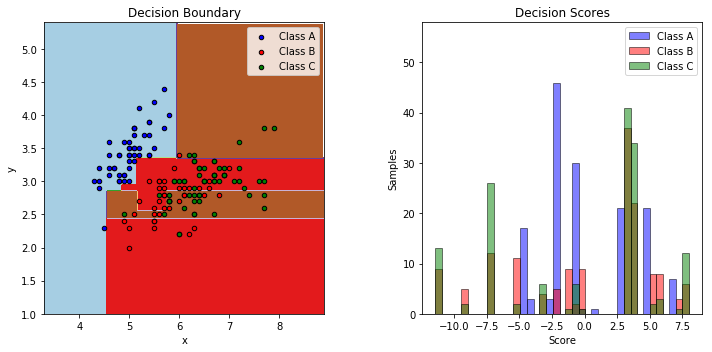
\includegraphics[width=0.8\textwidth]{ada_tree}
  \caption{对于采用决策树作为弱学习机的分类器在样本的两个特征上面训练出来的分类边界的可视化, 可以看到其保持了原弱学习机的分类特点, 可以说是一个超级纵横学习机.}
\end{figure}



\subsection{学习机数量提升}

%\todo{改个参数}

那么一个最简单的改进的思路就是去增加弱学习机的数量, 通过更大的学习规模去对函数做更好的拟合. 那么我们在增加学习机的规模的时候并没有任何的效果上的提升. 甚至还有所下降. 通过简化版学习机的分类边界可视化, 我们不难观察到这样的增加弱学习机的数量并没有对我们的分类边界产生任何实质性的影响. 甚至都没有增加分类边界的曲折程度, 只是边的位置有了一定调整. 所以我们基本可以认为此时模型的限制基本完全来源于弱学习机的分类特点.


\begin{figure}[hbt]
\centering
  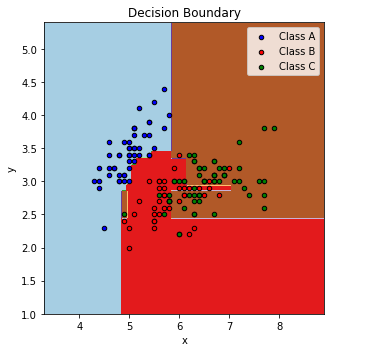
\includegraphics[width=0.45\textwidth]{adat50}
  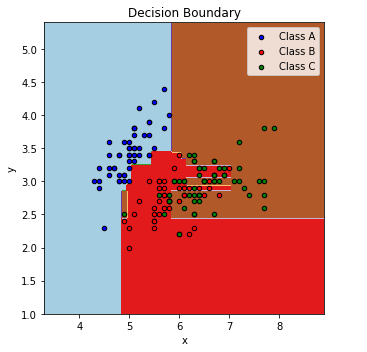
\includegraphics[width=0.45\textwidth]{adat100}\\
  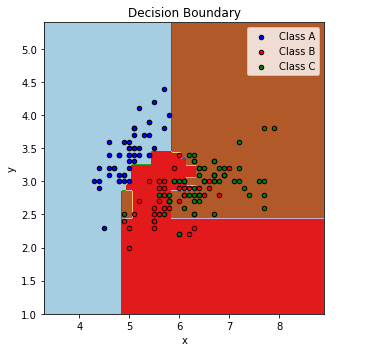
\includegraphics[width=0.45\textwidth]{adat150}
  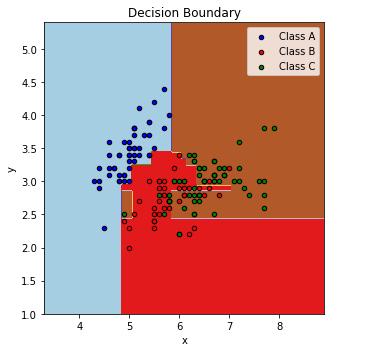
\includegraphics[width=0.45\textwidth]{adat200}
  \caption{我们的弱学习机数量从50增加到了100、150、200. 可以看到其并没有任何的明显的质变, 分类边界并没有变细腻, 只是边界的位置换了地方.}
\end{figure}



\subsection{支撑向量机弱学习机}

根据我们上面的分析, 结合Boosting过程的特性, 另外一个显然的想法就是尝试不同的弱学习机去提升我们的分类准确率. 我们又尝试了支撑向量机作为我们的弱学习机去进行Adaboosting学习. sklearn.svm类中的svc类给我们提供这样现成的弱学习机. 在支撑向量机里, 我们采用了线性的核函数. 通过使用相同的参数, 我们发现这样的弱学习机的选取也可以极大程度上的影响我们的分类准确率. 我们的分类准确率从87.6\%提升到了94.1\%. 几乎正确分对了绝大多数的测试集里的数据.

依旧我们对于两个特征又训练了一个模型用于可视化, 采用了同样的可视化方案, 我们发现了采用svm作为弱学习机的adaboost学习机与原来的采用决策树的有了质的改变.

\begin{figure}[hbt]	
\centering
  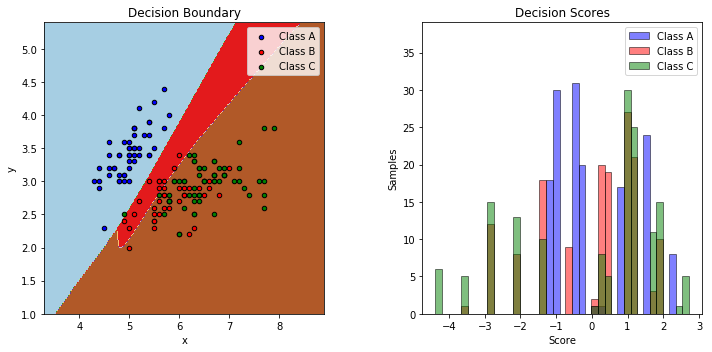
\includegraphics[width=0.8\textwidth]{svm50}
  \caption{采用了svm作为弱学习机的adaboost算法. 能够明显地以更简单的方式更好地捕捉类与累之间的边界.}
\end{figure}


并且可以从图上观察出我们的分类器的确能够相比采用决策树时更好地捕捉到类边界. 相比于决策树的边界而言, SVM作为弱学习机习得的边界不再是一条直线, 故显著增加了分类准确性. 我们还可以观察到在A类与B、C类的分离时几乎没有错分, 但是我们与上次一样依旧需要更多的信息去区分B、C类. 并且但我们在此时提高弱学习机数量的时候, 我们的分类边界也有了明显的变化. 其能够进一步地捕捉到类与类之间的边界. 我们在全样本四个特征上面的学习机的准确率也提升了两个百分点左右达到了95.9\%. 但是当我们再一次提高我们的弱学习机数量时, 我们就再也得不到任何的性能提升了, 二维特征训练出的学习机可视化的结果也保持了基本不变.

\begin{figure}[hbt]
  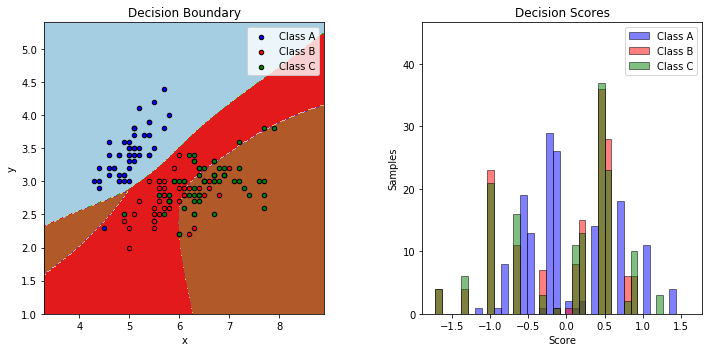
\includegraphics[width=0.8\textwidth]{svm100}
  \caption{弱SVM分类器的数量从50增加到100, 我们的二维特征上训练出来的学习机的分类性能得到了显著的改善, 能够进一步捕捉到数据的边界特征.}
\end{figure}



\newpage
\nocite{*}

% 如果想修改参考文献样式( 非国标 ), 请把下行取消注释, 并换成合适的样式( 比如 unsrt, plain 样式 ). 
\bibliographystyle{unsrt}
\bibliography{wpref}

\end{document}
